\documentclass{article}
\usepackage[utf8]{inputenc}
\usepackage{enumitem}
\usepackage{ulem}
\usepackage{mathrsfs}
\usepackage{amsmath}
\usepackage{float}
\usepackage{algorithm}
\usepackage{algpseudocode}
\usepackage{hyperref}
\usepackage{xcolor}
\usepackage{listings}
\usepackage{color}
\usepackage[utf8]{inputenc}
\usepackage{CJK}
\usepackage{amsthm,amsmath,amssymb}
\usepackage{hyperref}
\usepackage{relsize}
\usepackage{graphicx}
\usepackage{mathtools}
\usepackage{tikz}
\usepackage{bbm}

\newtheorem{problem}{Problem}

\newcommand{\N}{\mathcal N}
\newcommand{\Y}{\mathbf Y}
\newcommand{\real}{\mathbb{R}}
\newcommand{\X}{\mathbf X}
\newcommand{\Z}{\mathbf Z}

\newcommand*{\tran}{^{\mkern-1.5mu\mathsf{T}}}
\newcommand*{\hermitian}{^{\mkern-1.5mu\mathsf{H}}}

\newcommand{\Tau}{\mathrm{T}}

\DeclareMathOperator{\Tr}{Tr}

\def\Epsilon{E}
\def\Eta{H}

\def\veczero{{\mathbf 0}}
\def\vec1{{\mathbf 1}}
\def\matzero{{\mathbf 0}}

\def\veca{{\mathbf a}}
\def\vecb{{\mathbf b}}
\def\vecc{{\mathbf c}}
\def\vecd{{\mathbf d}}
\def\vece{{\mathbf e}}
\def\vecf{{\mathbf f}}
\def\vecg{{\mathbf g}}
\def\vech{{\mathbf h}}
\def\veck{{\mathbf k}}
\def\vecm{{\mathbf m}}
\def\vecn{{\mathbf n}}
\def\vecp{{\mathbf p}}
\def\vecq{{\mathbf q}}
\def\vecr{{\mathbf r}}
\def\vect{{\mathbf t}}
\def\vecu{{\mathbf u}}
\def\vecv{{\mathbf v}}
\def\vecw{{\mathbf w}}
\def\vecx{{\mathbf x}}
\def\vecy{{\mathbf y}}
\def\vecz{{\mathbf z}}

\def\vecalpha{{\mathbf \alpha}}
\def\vecbeta{{\mathbf \beta}}
\def\vecepsilon{{\boldsymbol \epsilon}}
\def\veclambda{{\mathbf \lambda}}
\def\vecvarepsilon{{\boldsymbol \varepsilon}}
\def\vecgamma{{\boldsymbol \gamma}}
\def\vecmu{{\boldsymbol \mu}}
\def\vecnu{{\boldsymbol \nu}}
\def\vecomega{{\boldsymbol \omega}}
\def\vecphi{{\boldsymbol \phi}}
\def\vecpsi{{\boldsymbol \psi}}
\def\vecsigma{{\mathbf \sigma}}
\def\vecvarsigma{{\mathbf \varsigma}}
\def\vectau{{\boldsymbol \tau}}
\def\vecupsilon{{\boldsymbol \upsilon}}
\def\vecvarphi{{\boldsymbol \varphi}}
\def\vecxi{{\boldsymbol \xi}}
\def\veczeta{{\boldsymbol \zeta}}


\def\vecX{{\mathbf X}}
\def\vecY{{\mathbf Y}}
\def\vecZ{{\mathbf Z}}

\def\vecEpsilon{{\mathbf \Epsilon}}
\def\vecEta{{\mathbf \Eta}}


\def\matA{{\mathbf A}}
\def\matB{{\mathbf B}}
\def\matC{{\mathbf C}}
\def\matD{{\mathbf D}}
\def\matE{{\mathbf E}}
\def\matF{{\mathbf F}}
\def\matH{{\mathbf H}}
\def\matI{{\mathbf I}}
\def\matK{{\mathbf K}}
\def\matL{{\mathbf L}}
\def\matO{{\mathbf O}}
\def\matOmega{{\mathbf \Omega}}
\def\matN{{\mathbf N}}
\def\matP{{\mathbf P}}
\def\matS{{\mathbf S}}
\def\matU{{\mathbf U}}
\def\matV{{\mathbf V}}
\def\matW{{\mathbf W}}
\def\matX{{\mathbf X}}
\def\matZ{{\mathbf Z}}
\def\matGamma{{\mathbf{\mathrm{\Gamma}}}}
\def\matLambda{{\mathbf{\mathrm{\Lambda}}}}
\def\matOmega{{\mathbf{\mathrm{\Omega}}}}
\def\matPhi{{\mathbf \Phi}}
\def\matPsi{{\mathbf \Psi}}
\def\matRho{{\mathbf{\mathrm{P}}}}
\def\matSigma{{\mathbf{\mathrm{\Sigma}}}}
\def\matUpsilon{{\mathbf{\mathrm{\Upsilon}}}}
\def\matXi{{\mathbf{\mathrm{\Xi}}}}

\def\matzero{{\mathbf 0}}


\def\complex{{\mathbb {C}}}
\def\real{{\mathbb {R}}}
\def\extreal{\overline{\mathbb {R}}}
\def\rational{{\mathbb {Q}}}
\def\pnint{{\mathbb {Z}}}
\def\nnint{{\mathbb{N}_0}}
\def\pint{{\mathbb {N}}}
\def\extint{\overline{\mathbb {Z}}}

\def\defas{:=}
\def\as{\overset{\mbox{a.s.}}{=}}
\def\ind{1}
\def\normal{\calN}
\def\expect{\mathbb{E}}
\def\variance{\mbox{Var}}
\def\covariance{\mbox{Cov}}
\def\prob{\mathbb{P}}
\def\risk{\calR}
\def\Uniform{{\cal{U}}}
\def\Trace{\mbox{Tr}}
\def\sign{\mbox{sign}}
\def\evaloss{\star}
\def\margin{\varrho}
\def\Log{{Log}}

\def\converged{\xrightarrow[]{D}}
\def\convergep{\xrightarrow[]{P}}
\def\convergeas{\xrightarrow[]{a.s.}}

\def\Borel{{\frakB}}

\def\Re{\mbox{Re}}
\def\Im{\mbox{Im}}

\def\interior{\mathrm{o}}

\def\calA{{\cal A}}
\def\calB{{\cal B}}
\def\calC{{\cal C}}
\def\calD{{\cal D}}
\def\calE{{\cal E}}
\def\calF{{\cal F}}
\def\calG{{\cal G}}
\def\calH{{\cal H}}
\def\calK{{\cal K}}
\def\calL{{\cal L}}
\def\calM{{\cal M}}
\def\calN{{\cal N}}
\def\calP{{\cal P}}
\def\calR{{\cal R}}
\def\calS{{\cal S}}
\def\calT{{\cal T}}
\def\calV{{\cal V}}
\def\calX{{\cal X}}
\def\calY{{\cal Y}}
\def\calZ{{\cal Z}}

\def\scrA{\mathscr{A}}
\def\scrB{\mathscr{B}}
\def\scrC{\mathscr{C}}
\def\scrD{\mathscr{D}}
\def\scrE{\mathscr{E}}
\def\scrF{\mathscr{F}}
\def\scrG{\mathscr{G}}
\def\scrI{\mathscr{I}}
\def\scrJ{\mathscr{J}}
\def\scrK{\mathscr{K}}
\def\scrL{\mathscr{L}}
\def\scrM{\mathscr{M}}
\def\scrN{\mathscr{N}}
\def\scrP{\mathscr{P}}
\def\scrQ{\mathscr{Q}}
\def\scrR{\mathscr{R}}
\def\scrS{\mathscr{S}}
\def\scrU{\mathscr{U}}
\def\scrV{\mathscr{V}}
\def\scrX{\mathscr{X}}


\def\pzch{\mathpzc{h}}
\def\pzcy{\mathpzc{y}}

\def\frakA{\mathfrak{A}}
\def\frakB{\mathfrak{B}}
\def\frakG{\mathfrak{G}}
\def\frakM{\mathfrak{M}}

\def\continuous{{\cal C}}


\addtolength{\oddsidemargin}{-.875in}
\addtolength{\evensidemargin}{-.875in}
\addtolength{\textwidth}{1.75in}
\addtolength{\topmargin}{-.875in}
\addtolength{\textheight}{1.75in}


\title{HW4 Handwritten Assignment}
\author{Lecturor: Pei-Yuan Wu\\
TAs: {Chun-Lin Huang(Problem 1, 2), Yuan-Chia Chang(Problem 3, 4, 5)}}
\date{November 2023, Sixth Edition}
\begin{document}

\maketitle

\section*{Problem 1 (EM algorithm for mixture of Bernoulli model)(1.5\%)}
Consider the generative model parameterized by $\theta = (\pi_k,\vecmu_k)_{k=1}^K$, where $\pi_1,...,\pi_K \in [0,1]$ satisfies $\sum_{k=1}^K\pi_k = 1$, and that $\vecmu_1,...,\vecmu_K  \in [0,1]^D$, so that the probability of generating a $D$-dimensional binary vector $\vecx = (x^{(1)},...,x^{(D)}) \in \{0,1\}^D$ is
\begin{equation*}
p(\vecx; \theta) = \sum_{k=1}^K \pi_k \prod_{j=1}^D \mu_{kj}^{x^{(j)}}(1-\mu_{kj})^{1-x^{(j)}}
\end{equation*}
%
In other words, with given $\vecmu_k$, the elements $x^{(1)},...,x^{(D)}$ are independent, where $x^{(j)}$ follows Bernoulli distribution of mean $\mu_{kj}$.  Suppose we observe training data of $N$ binary vectors $\vecx_1,...,\vecx_N \in \{0,1\}^D$, derive the E-step and M-step equations of the EM algorithm for optimizing the mixing coefficients $\pi_k$ and the Bernoulli means $\mu_{kj}$ by maximum likelihood.

\section*{Problem 2 (EM algorithm for mixture of exponential model)(1.5\%)}
Given N samples \(x_{1},\ldots,x_{N} \in \lbrack 0,\infty)\), we would
like to cluster them into \(K\) clusters. Assume the samples are
generated according to Exponential mixture models
\[X\sim\sum_{j = 1}^{K}{\pi_{j}Exp(\tau_{j})}\]
where \(\pi_{1} + \ldots + \pi_{K} = 1\), and \(Exp(\tau)\) denotes the
exponential distribution with probability density function
\[f_{\tau}(x) = \left\{ \begin{matrix}
\begin{matrix}
(1/\tau)e^{- x/\tau} & ,\ x \geq 0 \\
\end{matrix} \\
\begin{matrix}
0\ \ \ \ \ \ \ \  & ,x < 0 \\
\end{matrix} \\
\end{matrix} \right.\ \]


We would like to apply Expectation Maximization algorithm to find the
maximum likelihood estimation of parameters
\(\theta = \left\{ (\pi_{k},\tau_{k}) \right\}_{k = 1}^{K}\).
\begin{enumerate}[label=(\alph*)]
\item
   Please write down the E-step and M-step and show
  that the parameters are updated from
  \(\theta^{(t)} = \left\{ (\pi_{k}^{(t)},\tau_{k}^{(t)}) \right\}_{k = 1}^{K}\)
  to
  \(\theta^{(t + 1)} = \left\{ (\pi_{k}^{(t + 1)},\tau_{k}^{(t + 1)}) \right\}_{k = 1}^{K}\)
  in the following form:

\[\tau_{k}^{(t + 1)} = \frac{\sum_{i = 1}^{N}{\delta_{ik}^{(t)}x_{i}}}{\sum_{i = 1}^{N}\delta_{ik}^{(t)}},\ \ \pi_{k}^{(t + 1)} = \frac{1}{N}\sum_{i = 1}^{N}\delta_{ik}^{(t)}\]

\item
  What is the closed form expression of
  \(\delta_{ik}^{(t)}\)?
\end{enumerate}


\section*{Problem 3 (Boosting)(0.5\%)}
\begin{enumerate}
\item  Consider training a boosting classifier using decision stumps on the data set illustrated in Figure \ref{fig:adaboost_toy_example}:
	\begin{figure}[H]
	\centerline{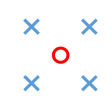
\includegraphics[width = 2 cm, height = 2 cm]{adaboost_toy_example.png}}
	\caption{
	AdaBoost Data set
	}
	\label{fig:adaboost_toy_example}
	\end{figure} 
	%
	\begin{enumerate}
	\item Which examples will have their weights increased at the end of the first iteration? Circle them.
	\item  How many iterations will it take to achieve zero training error? Justify your answers.
	\end{enumerate}
	%
\item  Suppose AdaBoost is run on $N$ training examples, and suppose on each round that the weighted training error $\epsilon_t$ of the $t$'th weak hypothesis is at most $1/2-\gamma$, for some number $0 < \gamma < 1/2$. After how many iterations, $T$, will the combined hypothesis be consistent with the $N$ training examples, i.e., achieves zero training error? Your answer should only be expressed in terms of $N$ and $\gamma$. (Hint: Recall that exponential loss is an upper bound for 0-1 loss. What is the training error when $1$ example is misclassified?)
\end{enumerate}

\section*{Problem 4 (Expectation Maximization Interpretation behind Semi-Supervised Learning)(1\%)}

Given N samples
\(\mathbf{x}_{1},\ldots,\mathbf{x}_{N} \in \mathbb{R}^{m}\) as well as
their labels \(y_{1},\ldots,y_{N} \in \left\{ 0,1,\ldots,K \right\}\).
Consider the generative model where each sample \(\mathbf{x}_{i}\) is
generated independently according to Gaussian mixture model
\emph{\uline{that depends on the label \(y_{i}\)}}, as represented by
random variable

\[X_{i}\sim\left\{ \begin{matrix}
\begin{matrix}
\sum_{j=1}^{K}{\pi_{j}\mathcal{N}\left( \vecmu_{j},\mathbf{\Sigma}_{j} \right)} & ,\ if\ y_{i} = 0 \\
\end{matrix} \\
\begin{matrix}
\mathcal{N}\left( \vecmu_{k},\mathbf{\Sigma}_{k} \right) & ,\ if\ y_{i} = k \neq 0 \\
\end{matrix} \\
\end{matrix} \right.\ \]

where \(\pi_{1} + \ldots + \pi_{K} = 1\), and
\(\mathcal{N}\left( \vecmu,\mathbf{\Sigma} \right)\) denotes the
Gaussian distribution with mean \(\vecmu\) and covariance matrix
\(\mathbf{\Sigma}\), with probability density function

\[\mathcal{N}\left( \mathbf{x};\vecmu,\mathbf{\Sigma} \right) = \frac{1}{\sqrt{(2\pi)^{m}\left| \mathbf{\Sigma} \right|}}\exp\left( - \frac{1}{2}\left( \mathbf{x - \vecmu} \right)^{T}\mathbf{\Sigma}^{- 1}\left( \mathbf{x - \vecmu} \right) \right)\]

We would like to apply Expectation Maximization algorithm to find the
maximum likelihood estimation of parameters
\(\theta = \left\{ (\pi_{k},\vecmu_{k},\mathbf{\Sigma}_{k}) \right\}_{k = 1}^{K}\).

\begin{enumerate}
\item
Please write down the E-step and M-step and show
  that the parameters are updated from \\
  \(\theta^{(t)} = \left\{ \left( \pi_{k}^{(t)},\vecmu_{k}^{(t)},\mathbf{\Sigma}_{k}^{(t)} \right) \right\}_{k = 1}^{K}\)
  to
  \(\theta^{(t + 1)} = \left\{ \left( \pi_{k}^{(t + 1)},\vecmu_{k}^{(t + 1)},\mathbf{\Sigma}_{k}^{(t + 1)} \right) \right\}_{k = 1}^{K}\)
  in the following form:


\[\pi_{k}^{(t + 1)} = \frac{\sum_{i:y_{i} = 0}^{}\delta_{ik}^{(t)}}{\sum_{i:y_i=0}1}\]

\[\vecmu_{k}^{(t + 1)} = \frac{\sum_{i:y_{i} = k}^{}\mathbf{x}_{i} + \sum_{i:y_{i} = 0}^{}{\delta_{ik}^{(t)}\mathbf{x}_{i}}}{N_{k} + \sum_{i:y_{i} = 0}^{}\delta_{ik}^{(t)}}\]

\[\mathbf{\Sigma}_{k}^{(t + 1)} = \frac{\sum_{i:y_{i} = k}^{}{\left( \mathbf{x}_{i} - \vecmu_{k}^{(t + 1)} \right)\left( \mathbf{x}_{i} - \vecmu_{k}^{(t + 1)} \right)^{T}} + \sum_{i:y_{i} = 0}^{}{\delta_{ik}^{(t)}\left( \mathbf{x}_{i} - \vecmu_{k}^{(t + 1)} \right)\left( \mathbf{x}_{i} - \vecmu_{k}^{(t + 1)} \right)^{T}}}{N_{k} + \sum_{i:y_{i} = 0}^{}\delta_{ik}^{(t)}}\]

\begin{quote}
where \(N_{k} = \sum_{i:y_{i} = k}^{}1\) is the number of samples in
class k. Please show your derivations.
\end{quote}

\item
 What is the closed form expression of
  \(\delta_{ik}^{(t)}\)? Please show your derivations.
\end{enumerate}

\section*{Problem 5 (Label Propagation Algorithm)(1.5\%)}

In this problem, we will investigate label propagation algorithm by executing on a toy example. Next, we will show that the algorithm will convergence, which can be expressed analytically.

Let's consider the graph that we have seen in HW3 Problem 2.

\begin{figure}[ht!]
        \centering
    \begin{tikzpicture}[main/.style = {draw, circle}]
    \node[main] (1) [color=red] {$x_1$}; 
    \node[main] (2) [below right of=1] {$x_2$}; 
    \node[main] (3) [below left of=1] {$x_3$}; 
    \node[main] (4) [above right of=1] {$x_4$}; 
    \node[main] (9) [below left of=3] {$x_9$}; 
    \node[main] (10) [below right of=3] {$x_{10}$}; 
    \node[main] (8) [above of=4] {$x_8$}; 
    \node[main] (7) [color=blue] [below right of=10] {$x_7$}; 
    \node[main] (5) [right of=7] {$x_5$}; 
    \node[main] (6) [right of=5] {$x_6$};
    \draw (1) -- (2); 
    \draw (1) -- (3); 
    \draw (1) -- (4);
    \draw (2) -- (4); 
    \draw (2) to [out=45,in=45,looseness=1.5]  (8);
    \draw (3) to [out=135,in=135,looseness=1.5]  (8);
    \draw (5) -- (6); 
    \draw (5) -- (7); 
    \draw (7) -- (10); 
    \draw (8) to [out=90,in=180,looseness=3]  (9);
    \draw (9) -- (10); 
    \end{tikzpicture}
        \caption{undirected connected graph $G$ with labeled node}
    \end{figure}

We have previously known that $x_1$ node is in Class 1 and $x_7$ node is in Class 2. Now, we want to separate these 10 nodes into Class 1 and Class 2.

Consider the transition matrix $\boldsymbol{T}$,
$$\boldsymbol{T}_{i,j} = \frac{\boldsymbol{\Tilde{W}}_{i,j}}{\sum_{k=1}^{10} \boldsymbol{\Tilde{W}}_{k,j}}$$,
where $\boldsymbol{\Tilde{W}}$ is the adjusted adjacency matrix of the graph G, which is defined as 
$$\boldsymbol{\Tilde{W}} = \boldsymbol{W} + \delta
\begin{bmatrix}
    1 & 1 & \dots  & 1 \\
    1 & 1 & \dots  & 1 \\
    \vdots & \vdots & \ddots & \vdots \\
    1 & 1 &  \dots  &  1
\end{bmatrix}$$. $\delta > 0$ is a small number. By adjusting the adjacency matrix, the weight of edge being connected in the original graph G is $1+\delta$ and the weight of other edges is $\delta$. Through the adjustment, we can prevent that the algorithm runs unsupervised due to the isolated labeled nodes. In the toy example, we set $\delta=0.01$.  
$\boldsymbol{T}_{i,j}$ represents the probability that node $j$ will propagate its own state to node $i$. For example, $\boldsymbol{T}_{2,1} = \boldsymbol{T}_{3,1} = \boldsymbol{T}_{4,1} \approx 0.326 \approx \frac{1}{3}, \boldsymbol{T}_{1,1} = \boldsymbol{T}_{5,1} = \boldsymbol{T}_{6,1} = \boldsymbol{T}_{7,1}= \boldsymbol{T}_{8,1}= \boldsymbol{T}_{9,1}= \boldsymbol{T}_{10,1}\approx 0.003$, which shows that node 1 will transfer its label to three neighbors with probability around 1 over 3. Also, it will transfer its label to other nodes(including itself) with probability slightly greater than zero.

 \begin{enumerate}
\item Please write down the transition matrix $\boldsymbol{T}$.
\end{enumerate}

Next, we define the label matrix sequence $$\boldsymbol{Y}^t \in \mathbb{R}^{10 \times 2} \quad t=0,1,...$$ where the $i_{th}$ row of $\boldsymbol{Y}^t$ means the probability distribution of node $x_i$ at time $t$. In this example, $\boldsymbol{Y}^t_{i,1}$ means the probability that the node $x_i$ lies in Class 1 at time $t$, and $\boldsymbol{Y}^t_{i,2}$ means the probability that the node $x$ lies in Class 2 at time $t$. We initialize $\boldsymbol{Y}^0_{1,1}=1, \boldsymbol{Y}^0_{1,2}=0$ because $x_1$ is labeled as Class 1. Also, $\boldsymbol{Y}^0_{7,1}=0, \boldsymbol{Y}^0_{7,2}=1$ because $x_7$ is labeled as Class 2. For other nodes i,  we initialize $\boldsymbol{Y}^0_{i,1}=\boldsymbol{Y}^0_{i, 2}=0.5$.

After defining label matrix $\boldsymbol{Y}$ and transition matrix $\boldsymbol{T}$, we introduce the algorithm below: \\

\begin{algorithm}
  \caption{Label Propagation Algorithm in Toy Example}
  \label{alg:label_propagation_algorithm_in_toy_example}
  \hspace*{\algorithmicindent} \textbf{Input}  label matrix $\boldsymbol{Y}^0$, transition matrix $\boldsymbol{T}$, tolerance level $\epsilon$ \\
  \hspace*{\algorithmicindent} \textbf{Output} node $x_i \in $ \{Class 1, Class 2\} \quad $i=1,,,10$
  \begin{algorithmic}[1]
    \Procedure{Label Propagation}{$\boldsymbol{Y}^0$, $\boldsymbol{T}$, $\epsilon$=$10^{-8}$}
    \State t = 0
    \Repeat
        \State t = t + 1
        \State $\boldsymbol{Y}^{t}$ = $\boldsymbol{T} \boldsymbol{Y}^{t-1}$ \Comment{Random walk to its neighbor}
        \State $\boldsymbol{Y}^{t}_{i,j} = \boldsymbol{Y}^{t}_{i,j} / (\boldsymbol{Y}^{t}_{i,1} + \boldsymbol{Y}^{t}_{i,2}) \quad i=1,...,10, j=1,2$ \Comment{Normalize the probability distribution}
        \State $\boldsymbol{Y}^{t}_{1,1} = 1, \boldsymbol{Y}^{t}_{1,2} = 0,\boldsymbol{Y}^{t}_{7,1} = 0,\boldsymbol{Y}^{t}_{7,2} = 1$ \Comment{Clamp the labeled data}
    \Until{ $||\boldsymbol{Y}^{t}-\boldsymbol{Y}^{t-1}||_F < \epsilon$}
    \State If $\boldsymbol{Y}^{t}_{i,1} > 0.5$ then node $x_i$ lies in Class 1, otherwise node $x_i$ lies in Class 2, \quad $i=1,...,10$
    \EndProcedure
   \end{algorithmic}
\end{algorithm}

\newpage
There are three main procedures in the loop. First, every node propagates it own state to its neighbors with the transition probability. Next, we normalize the probability distribution for every node. In the last step, we clamp the probability distribution of the labeled data, which prevents the distribution of labeled data being influenced by unlabeled data and accelerates the convergence speed of the algorithm.
\begin{enumerate}[resume]
\item Please execute the algorithm. Write down the iteration number $t$, $\boldsymbol{Y}^{t}$, which nodes lies in Class 1 and which nodes lies in Class 2. Does the result correspond with the graph?
\end{enumerate}

To show the convergence of label propagation algorithm, we consider more general case as the following statement.

Let $(x_1, y_1),...,(x_l,y_l)$ be labeled data, where $y_i$ takes value in $ \{ 1,..,C \} $, which indicates that $x_i$ lies in Class $y_i$. Also, we have $u$ unlabeled data  $(x_{l+1}, y_{l+1}),...,(x_{l+u},y_{l+u})$, where $y_j$ is an unknown value, which lies in $\{ 1,...,C \}$. 

We can construct the transition matrix $\boldsymbol{T}$,
$$\boldsymbol{T}_{i,j} = \frac{\boldsymbol{\Tilde{W}}_{i,j}}{\sum_{k=1}^{l+u} \boldsymbol{\Tilde{W}}_{k,j}}$$,
where $\boldsymbol{\Tilde{W}}_{i,j} > 0, \quad i,j = 1,..., l+u$.

Also, we define the label matrix sequence $$\boldsymbol{Y}^t \in \mathbb{R}^{(l+u) \times C} \quad t=0,1,...$$ where the $i_{th}$ row of $\boldsymbol{Y}^t$ means the probability distribution of node $x_i$ at time $t$. $\boldsymbol{Y}^t_{i,j}$ means the probability that the node $x_i$ lies in Class $j$ at time $t$. For $\boldsymbol{Y}^0$, we clamp the first $l$ rows as following,
$$\boldsymbol{Y}^{t}_{i,j}= \mathbbm{1}\{y_i=j\} \quad i = 1,...,l, j = 1,...,C$$,
which indicates that $x_i$ must lies in Class $y_i$. For the other rows, we initialize
$$\boldsymbol{Y}^{t}_{i,j}= \frac{1}{C} \quad i = l+1,...,l+u, j = 1,...,C$$

We execute by the algorithm below.

\begin{algorithm}
  \caption{Generalized Label Propagation Algorithm}
  \label{alg:generalized_label_propagation_algorithm}
  \hspace*{\algorithmicindent} \textbf{Input}  label matrix $\boldsymbol{Y}^0$ and transition matrix $\boldsymbol{T}$ \\
  \hspace*{\algorithmicindent} \textbf{Output} $\boldsymbol{Y}^*$
  \begin{algorithmic}[1]
    \Procedure{Generalize Label Propagation}{$\boldsymbol{Y}^0$, $\boldsymbol{T}$, $t=0$}
    \Repeat
        \State t = t + 1
        \State $\boldsymbol{Y}^{t}$ = $\boldsymbol{T} \boldsymbol{Y}^{t-1}$ \Comment{Random walk to its neighbor}
        \State $\boldsymbol{Y}^{t}_{i,j} = \boldsymbol{Y}^{t}_{i,j} / \sum_{k=1}^{C} \boldsymbol{Y}^{t}_{i,k} \quad i=1,...l+u ,j=1,...,C$ \Comment{Normalize the probability distribution}
        \State $\boldsymbol{Y}^{t}_{i,j}= \mathbbm{1}\{y_i=j\} \quad i = 1,...,l, j = 1,...,C$ \Comment{Clamp the labeled data}
    \Until{$\boldsymbol{Y}^{t}$ converges to $\boldsymbol{Y}^{*}$} 
    \EndProcedure
   \end{algorithmic}
\end{algorithm}

\newpage
Once we get $\boldsymbol{Y}^{*}$, we can conclude that the unlabeled data $(x_i,y_i)$ belong to Class $y_i$, where
$$y_i= \text{arg}\,\max\limits_{\j}\ \boldsymbol{Y}^{*}_{i,j}$$

Next, we want to calculate $\boldsymbol{Y}^{*}$ analytically.

\begin{enumerate}[resume]
\item Please show that the line 4 and 5 in Algorithm 2 can be combined as
$$\boldsymbol{Y}^{t} = \boldsymbol{\overline{T}} \boldsymbol{Y}^{t-1}$$, where
$\boldsymbol{\overline{T}}_{i,j}=\boldsymbol{T}_{i,j}/\sum_{k=1}^{l+u} \boldsymbol{T}_{i,k}, i,j=1,...,l+u$.
\end{enumerate}
We split $\boldsymbol{\overline{T}}$ to 
$\begin{bmatrix}
\boldsymbol{\overline{T}}_{ll} & \boldsymbol{\overline{T}}_{lu}\\
\boldsymbol{\overline{T}}_{ul} & \boldsymbol{\overline{T}}_{uu}
\end{bmatrix}$, where $\boldsymbol{\overline{T}}_{ll} \in \mathbb{R}^{l \times l}, \boldsymbol{\overline{T}}_{uu} \in \mathbb{R}^{u \times u}$. Also, we split $\boldsymbol{Y}^{t}$ to

$\begin{bmatrix}
\boldsymbol{Y}^{t}_L \\
\boldsymbol{Y}^{t}_U
\end{bmatrix}$, where $\boldsymbol{Y}^{t}_L \in \mathbb{R}^{l}, \boldsymbol{Y}^{t}_U \in \mathbb{R}^{u}$

\begin{enumerate}[resume]
\item Please show that after an iteration,
$$ \boldsymbol{Y}^{t}_U = \boldsymbol{\overline{T}}_{uu} \boldsymbol{Y}^{t-1}_U + \boldsymbol{\overline{T}}_{ul} \boldsymbol{Y}^{t-1}_L, t = 1,2,...,$$
$$\boldsymbol{Y}^{t}_L =  \boldsymbol{Y}^{t-1}_L, t = 1, 2,...$$
\item From the above result, we let $\boldsymbol{Y}_L=\boldsymbol{Y}^{t}_L$ for any $t$. Show that for $t \geq 1$ 
$$ \boldsymbol{Y}^{t}_U = \boldsymbol{\overline{T}}_{uu}^t \boldsymbol{Y}_U^{0} + \sum_{i=1}^t \boldsymbol{\overline{T}}_{uu}^{i-1} \boldsymbol{\overline{T}}_{ul} \boldsymbol{Y}_L$$

\item Please show that $\sum_{j=1}^u \boldsymbol{\overline{T}_{uu}}_{i,j} = \gamma_i$, where $0 < \gamma_i < 1$, for $i=1,...,u$. Use the fact to derive $\sum_{j=1}^u  \boldsymbol{\overline{T}_{uu}^n}_{i,j} \leq \gamma^n$, for $ i=1,...,u$, where $\gamma = \max\limits_{i=1,...,u} \gamma_i $. Last, derive $\lim_{n\to\infty} \boldsymbol{\overline{T}_{uu}^n} = \boldsymbol{O}$.


\item Define $\boldsymbol{S}_n = \boldsymbol{I} + \boldsymbol{\overline{T}}_{uu} + \boldsymbol{\overline{T}}_{uu}^2 + ... + \boldsymbol{\overline{T}}_{uu}^{n-1}, \quad \boldsymbol{S}_n(\boldsymbol{I}-\boldsymbol{\overline{T}}_{uu}) = \boldsymbol{I} - \boldsymbol{\overline{T}}_{uu}^{n}$. Use the fact to show that  
$\lim_{n\to\infty}\boldsymbol{S}_n = (\boldsymbol{I}-\boldsymbol{\overline{T}}_{uu})^{-1}$. Combined all the result above, please show that $\boldsymbol{Y}^{*}_U = (\boldsymbol{I}-\boldsymbol{\overline{T}}_{uu}))^{-1}\boldsymbol{\overline{T}}_{ul} \boldsymbol{Y}_L$. \\
Hence, $\boldsymbol{Y}^{*}=
\begin{bmatrix}
\boldsymbol{Y}_L \\
\boldsymbol{Y}^{*}_U
\end{bmatrix}
$, which can be obtained analytically regardless of the initial value $\boldsymbol{Y}^0$.

\item Please calculate the analytical solution $\boldsymbol{Y}^{*}$ on the toy example above. Does the solution correspond to the iteration solution $\boldsymbol{Y}^{t}$?
\end{enumerate}

 \section*{Version Description}
 \begin{enumerate}
     \item First Edition: Finish Problem 1 to 5
     \item Second Edition: Revise the data description in Problem 5 Generalized Label Propagation.
     \item Third Edition: Revise Problem 5 to make the definition more robust.
     \item Fourth Edition: Fix small typo at Problem 5 (5) $\boldsymbol{Y}^0 \rightarrow \boldsymbol{Y}_U^0$
     \item Fifth Edition: Fix typo at Problem 5 (6)
      \item Sixth Edition: Problem 4: edit $\pi_k^{t+1}$ 
 \end{enumerate}
\end{document}